\documentclass[12pt,letterpaper]{article}

\usepackage[utf8]{inputenc}
\usepackage[T1]{fontenc}
\usepackage{amsmath}
\usepackage{amsfonts}
\usepackage{amssymb}
\usepackage{amsthm}
\usepackage[left=2cm,right=2cm,top=2cm,bottom=2cm,headheight=22pt]{geometry}
\usepackage{fancyhdr}
\usepackage{setspace}
\usepackage{lastpage}
\usepackage{graphicx}
\usepackage{caption}
\usepackage{subcaption}

\theoremstyle{definition}
\newtheorem{question}{Question}
\newtheorem{example}{Example}
\newtheorem{exercise}[question]{Exercise}
\newtheorem*{challenge}{Challenge}

\begin{document}

%Paramètres de mise en forme des paragraphes selon les normes françaises
\setlength{\parskip}{1ex plus 0.5ex minus 0.2ex}
\setlength{\parindent}{0pt}

%Paramètres relatifs aux en-têtes et pieds de page.
\pagestyle{fancy}
\lhead{Theron J Hitchman}
\chead{\Large Reading and Guided Practice \#1}
\rhead{Fall 2013}
\lfoot{\emph{Math and Decision Making}}
\cfoot{} 
\rfoot{\emph{\thepage\ of \pageref{LastPage}}}

\section*{Introduction}
In this assignment you will learn about ``picture hanging puzzles."
This is our first introduction to a \emph{topological} problem, that is, a problem belonging to the field mathematicians call \emph{topology}.

\section*{Goals}
At the end of this assignment, a student should be able to:
\begin{itemize}
\item describe what is meant by the (2 nail) picture hanging puzzle.
\item draw diagrams corresponding to various arrangements of hanging a picture across two nails.
\item write down a compact notation describing such a diagram.
\item reconstruct a diagram from the relevant notation.
\item (Perhaps?) Solve the 2 nail picture hanging puzzle.
\end{itemize}

\section*{Reading and Questions for 28 Aug}

The original picture hanging puzzle is due to A.~Spivak \cite{Spivak}.
(Our study of it is based partly on work by Demaine et al. \cite{Demaine})
Ordinarily one hands a framed picture by looping a wire over a nail, like so:
\begin{figure}[h]
    \centering
    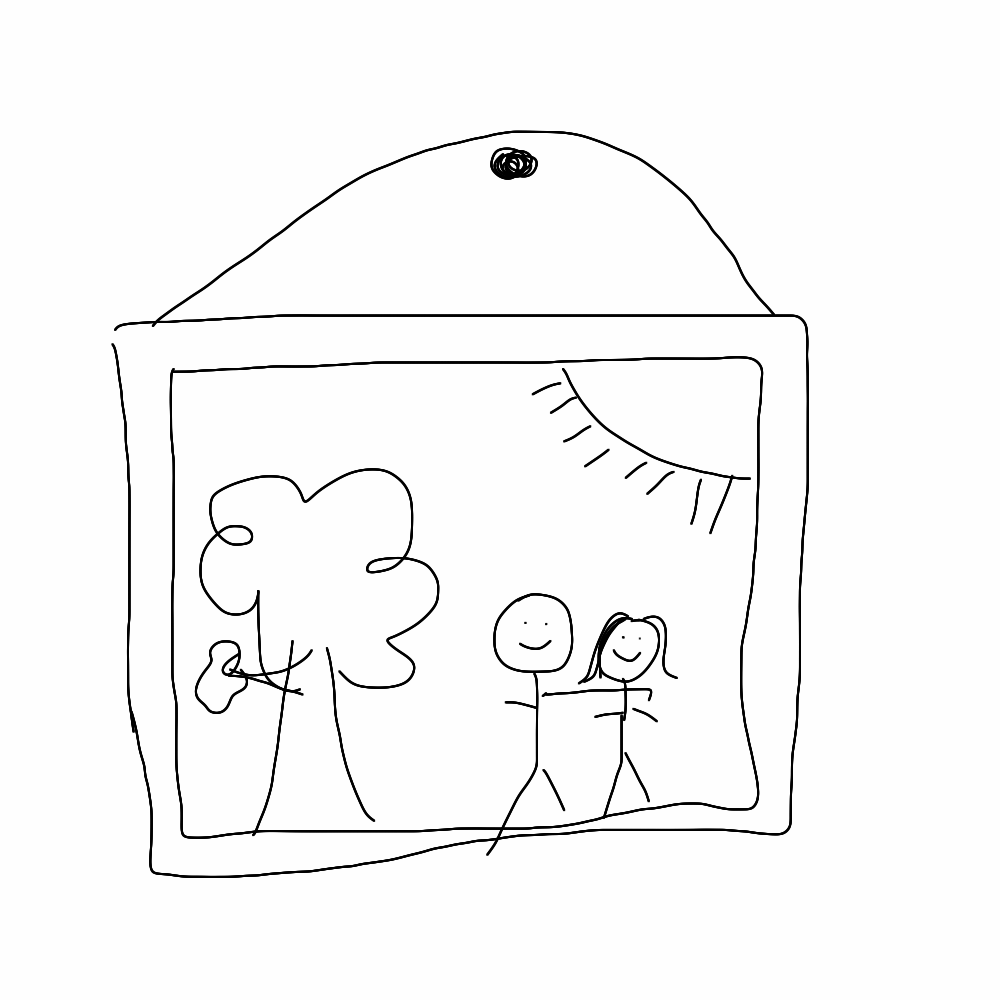
\includegraphics[height=3in]{rgp01pics/wedding.png}
    \caption{A photo from Prof H's wedding.}
\end{figure}
 
\clearpage
 
What if you had two nails, side-by-side? 
Most people would use an arrangment like this:
\begin{figure}[ht]
    \centering
    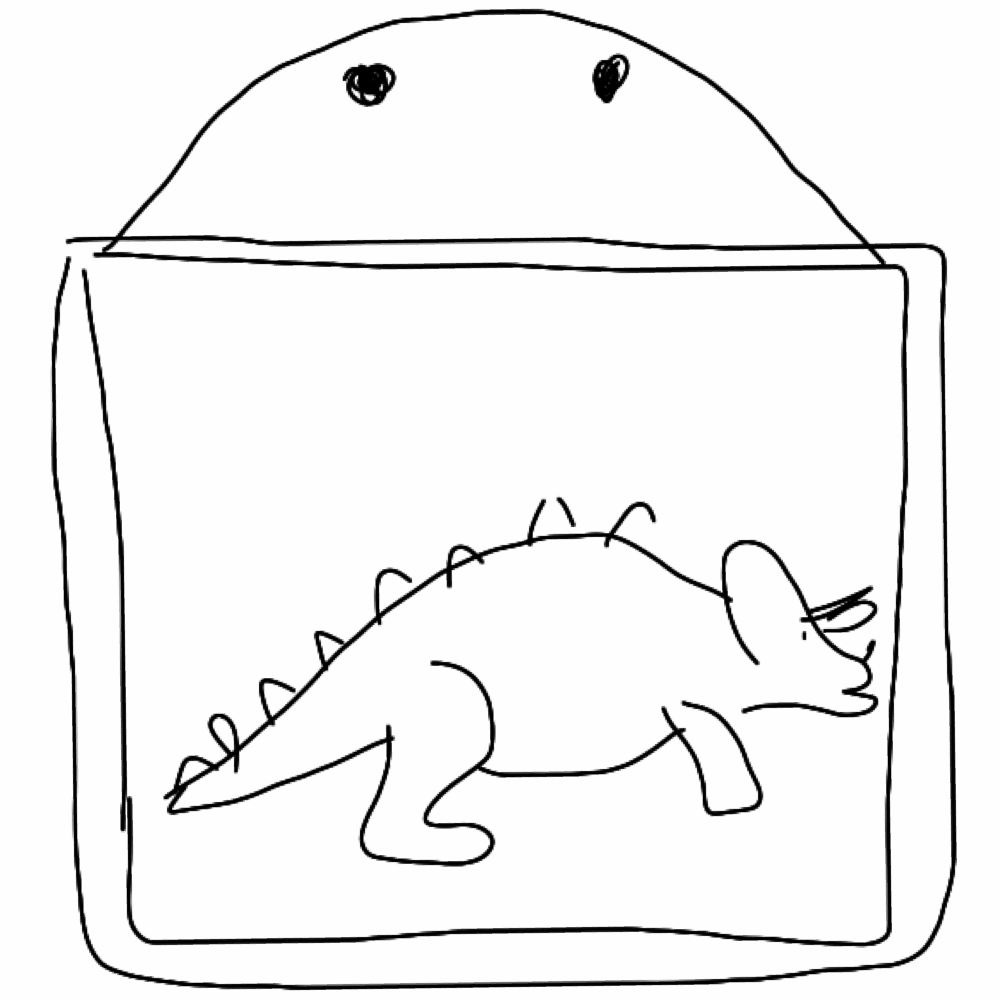
\includegraphics[height=2in]{rgp01pics/dinosaur}
    \caption{The framed picture is gone. But that is OK. We don't need it.}
\end{figure}

In this case, removing either nail doesn't make the picture fall down. 
It might hang crookedly, but it will stay on the wall.

\begin{quotation}
\textbf{2 Nail Picture Hanging Puzzle (PHP2)}\\
Is there a way to arrange the wire around the two nails so that
\begin{enumerate}
\item with both nails, the picture hangs from the wall, but
\item if \textbf{either} nail is removed, the picture will fall down?
\end{enumerate}
\end{quotation}

Our big goal for the week is to understand and solve this problem and some others like it.

We start by replacing the idea of a picture hanging by a wire from two nails with a curve snaking around two big dots.
The curve represents the wire and the big dots represent the two nails.
This is like imagining that you are looking straight at your materials, so the dots are really the nail heads.

\begin{question}
For each of the following three arrangements, which nail removals cause the picture to fall down?
For convenience, I have labelled the nails $A$ and $B$ so we can tell them apart.
\begin{figure}[h!]
    \centering
    \begin{subfigure}[b]{0.3\textwidth}
        \centering
        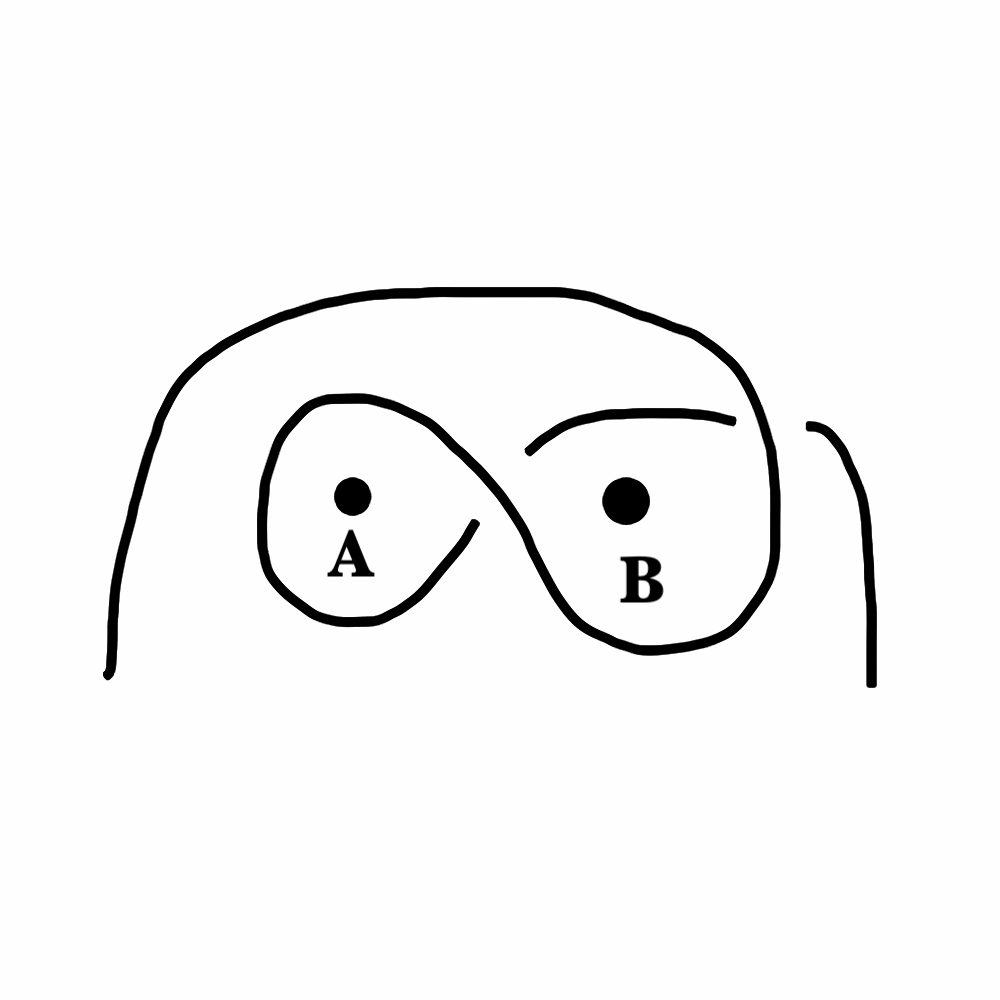
\includegraphics[width=\textwidth]{rgp01pics/attempt1.png}
        \caption{Attempt 1}
    \end{subfigure}
    \begin{subfigure}[b]{0.3\textwidth}
        \centering
        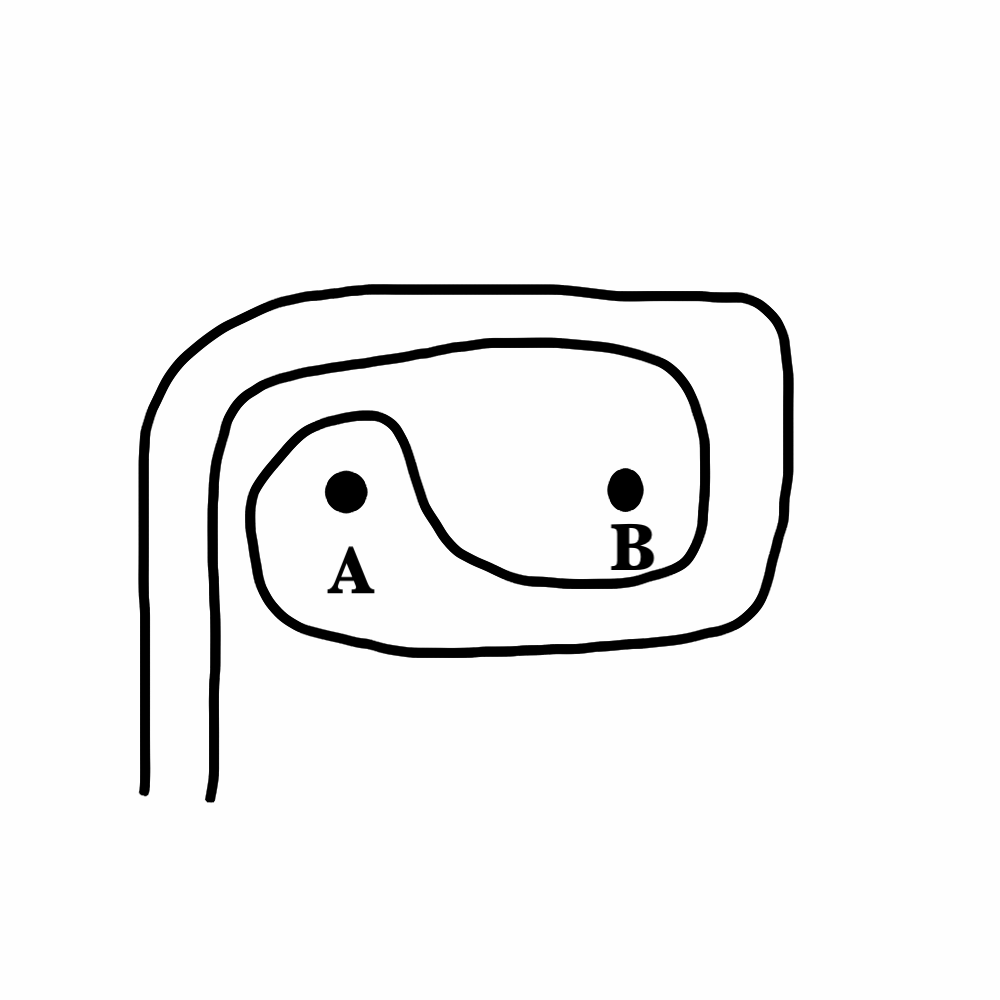
\includegraphics[width=\textwidth]{rgp01pics/attempt2.png}
        \caption{Attempt 2}
    \end{subfigure}
    \begin{subfigure}[b]{0.3\textwidth}
        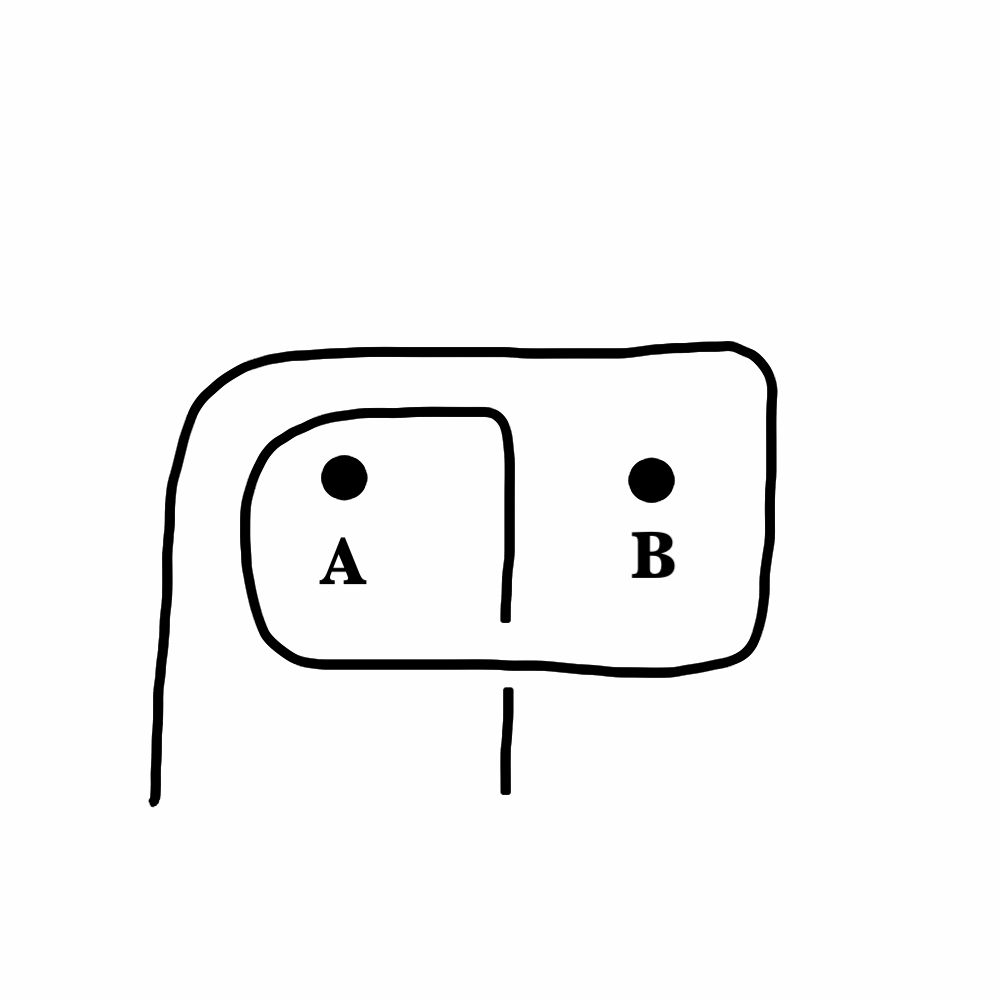
\includegraphics[width=\textwidth]{rgp01pics/attempt3.png}
        \caption{Attempt 3}
    \end{subfigure}
    \caption{Three Attempts to Solve PHP2}
\end{figure}
\end{question}

We have abstracted away the picture, and turned the nails into dots and the wire into a curve on the page, but more is possible.
Next we will further abstract away the pictures by introducing some symbols.

Here a string of symbols will represent a particular wrapping of the wire (i.e. a path of the curve around the dots).
The basic set up uses just the symbols for the nails!

\noindent
Step 1: Pick a ``direction of travel'' along the curve representing the wire.

\noindent
Step 2: As you pass \underline{over} a nail, you add a symbol which tells you the name of the nail and whether you are currently traveling left-to-right, or right-to-left. A symbol used by itself means left-to-right, a symbols with an asterisk on it means right-to-left.

Note: you ignore any time you pass under a nail. Only going over counts.

\begin{example}
In Attempt 1, start on the left hand side.
\begin{figure}[h]
    \centering
    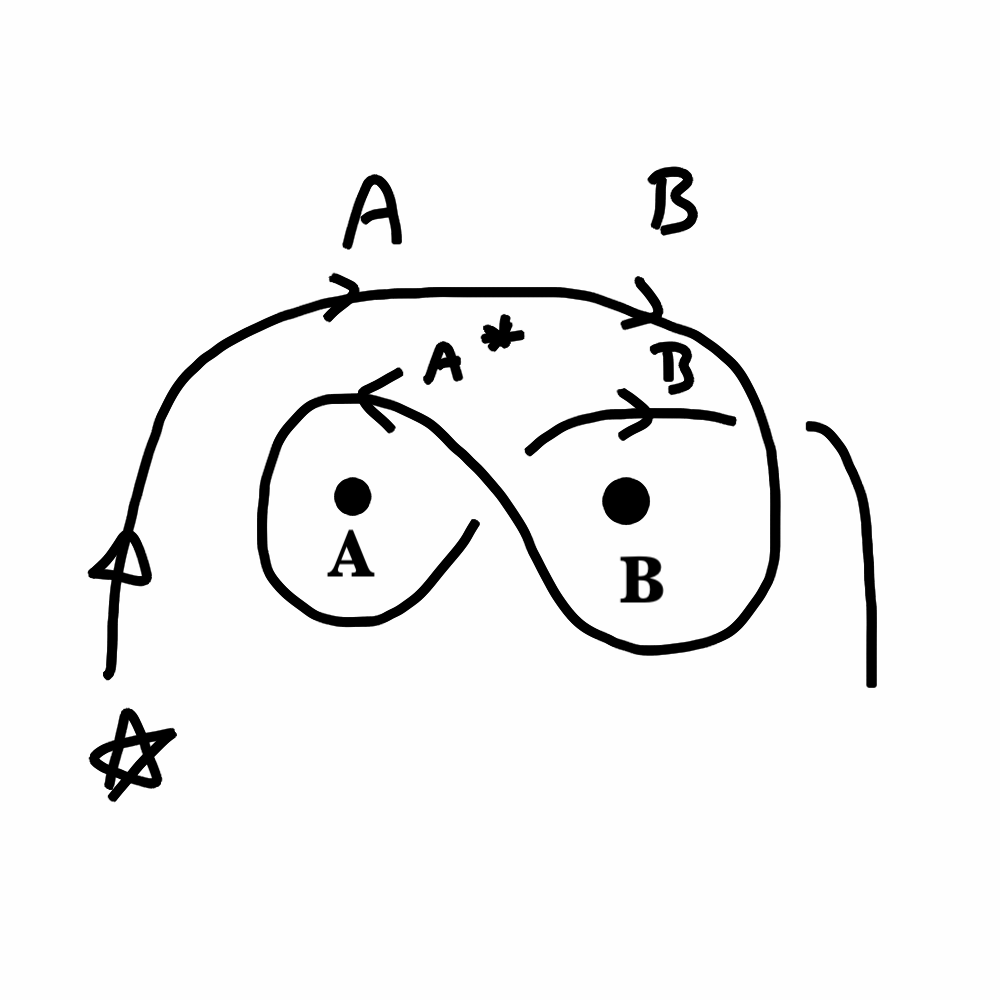
\includegraphics[height=3in]{rgp01pics/coded.png}
    \caption{Attempt 1, with important labels.}
\end{figure}
Then you do the following: (trace along with your finger)\\
\begin{center}
\begin{tabular}{lc}
the curve goes... & symbol \\
\hline
over A left to right & $A$\\
over B left to right & $B$\\
under B & --- \\
over A right to left & $A^*$\\
under A & --- \\
over B left to right & $B$ 
\end{tabular}
\end{center}
So in the end this diagram gets the symbol $ABA^*B$.
\end{example}

Now it is your turn to try.
\begin{exercise}
Check that if you start on the left-hand string in Attempt 2 the resulting symbol is $ABAB^*A^*$.
\end{exercise}

\begin{question}
What is the symbol for Attempt 3? Again, start with the left-hand string.
\end{question}

This whole process can work the other way, too.
If we take a string of the symbols $A$, $B$, $A^*$ and $B^*$, we can make a diagram with that symbol.
\begin{example} 
Consider the symbol $BABB$.
This has the following diagram:
\begin{figure}[h]
    \centering
    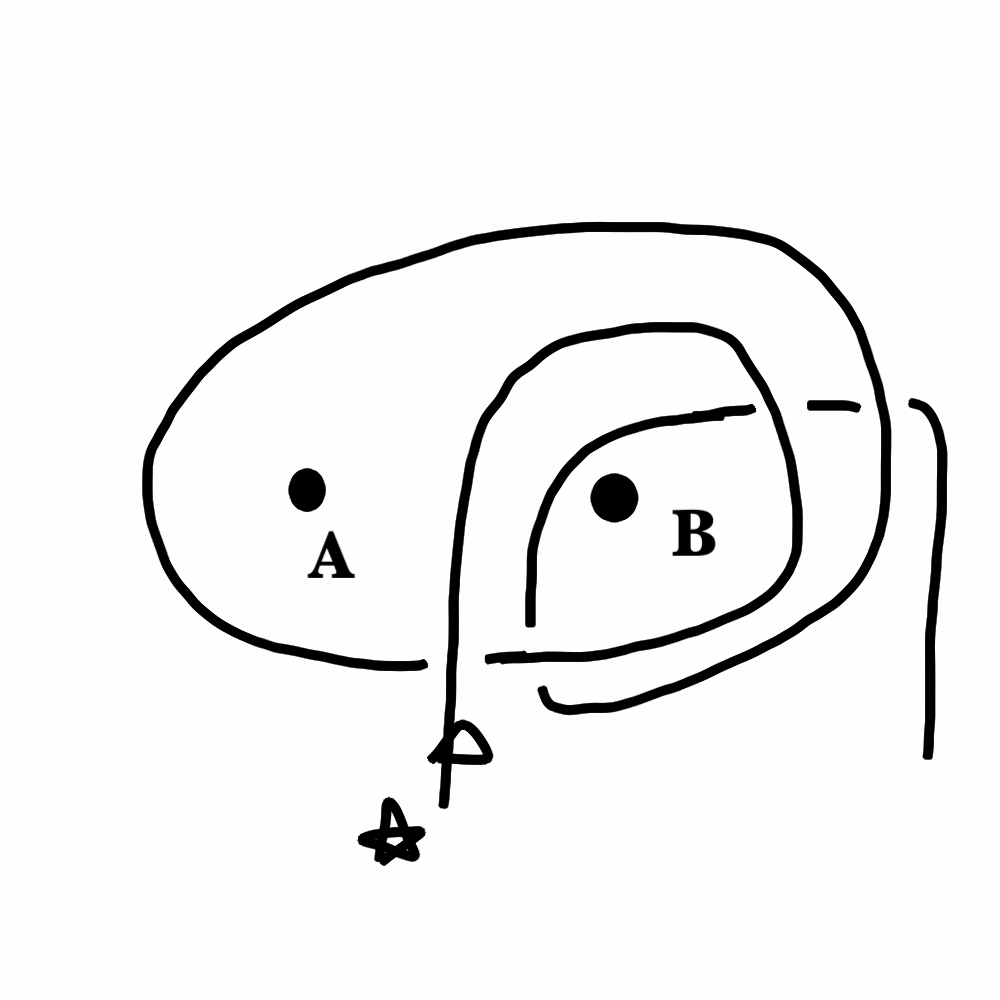
\includegraphics[height=3in]{rgp01pics/code2diagr.png}
    \caption{The diagram corresponding to $BABB$.}
\end{figure}
\end{example}

\begin{exercise} Make up 3 different symbols of your own and draw the corresponding diagrams.
Double check your work by reading back the symbol from your picture.\\
(Psst. Hey. Do any of your symbols happen to solve the picture hanging puzzle?)
\end{exercise}

\begin{challenge}
Now that you have a new way to organize things, can you solve the 2 nail picture hanging puzzle?
\end{challenge}

\begin{thebibliography}{9}

\bibitem{Spivak}
    A.~Spivak,
    Brainteasers B201: Strainge painting.
    \emph{Quantum}, page 13,
    May/June 1997

\bibitem{Demaine}
    Erik Demaine, Martin Demaine, Yair Minsky, Joseph Mitchell, Ronald Rivest, \& Mihai Patrascu,
    Picture Hanging Puzzles,
    available online at the arXiv: 1203.3602v1,
    16 March 2012
 
 \end{thebibliography}

\end{document}








